\chapter{Design and implentation}
The market app should be easy to use and fit for consumers of all ages. To install an application the user has to select a desired application with one touch, then check the specification if its compatible with the Arduino, then a agree/install button for installing the app on the Arduino. This is a total of two clicks, despite you have chosen a category or search hits on the market app. This is similar to Google Play.\\
\newline
Each (supported) Arduino device is equipped with a Unified Resource Identifier (URI) stored in its ROM. This URI is automatically transferred to the market app once it is turned on and is in range; the hardware configuration (Memory, connected devices) is stored in a XML file the URI links to.
The app store client can then compare compatibility with the device and app requirements.
Only apps supported on your Arduino will initially be visible in the market application, however, power users can enable unfiltered results to browse the selection and consider upgrading the device.\\
\newline
Anyone modifying a board will have to provide a hardware specification and transfer a new URI to the device if they want filtered results in the app store (Such a user could still choose to view and install unfiltered applications).
The URI could also be read from a QR-code.

\section{System Architecture}
	The design was divided into several modules:
	\begin{itemize}
		\item{Bluetooth connection between the Android and the Arduino}
		\item{Synchronization with the local SQLite database}
		\item{Android application view (the visible design)}
		\item{A service that contains the protocol for installing ``over the air''}
	\end{itemize}
	\vspace{0.2in}
	
	The system design was implemented such that further developing and extension should be as modular and easy as possible.
	Therefore it is designed as a plugin-like system where you easily can implement your own protocols against a desired device, e.g Raspberry Pi. The application only support STK500 protocol and therefore only connection towards Arduino.
	The design for the connection to other devices are done as following:\\

	\begin{figure}[H]
	\centering
	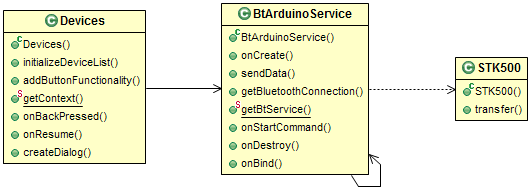
\includegraphics[width=130mm]{images/BTConnection.png}
	\end{figure}

	Devices.java is an Activity and can therefore be considered as a view in the application. To add a new service there is few changes to be done in Devices.java. Afterall an own service and a protocol towards a desired device must be implemented. Since this project only take in hand a connection between Android and Arduino, we implemented the STK500 protocol.
	The overall design solution for multiple connections will be like this:\\

	\begin{figure}[H]
	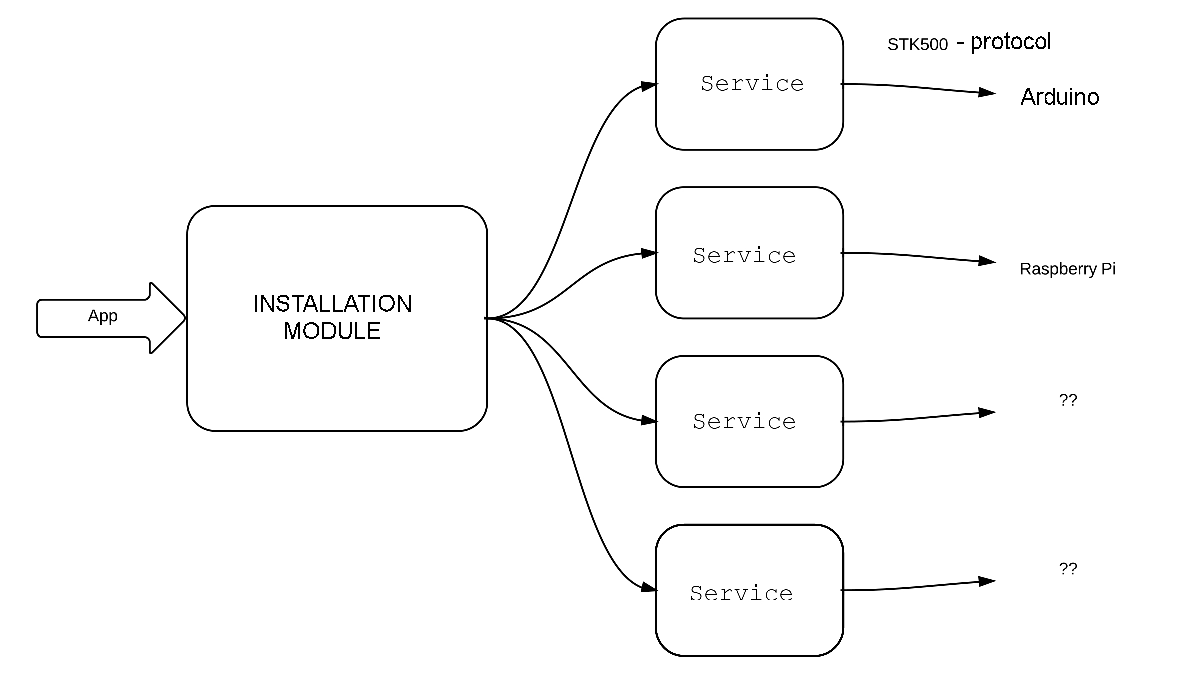
\includegraphics[scale=0.2]{figures/OTAArchitecture.pdf}
	\caption{Over The Air Architecture}
	\end{figure}

\section{Design of Android application}

% Add short description about what the purpose of the application is?

Before the programming of the Android application was started, a complete design guide were created. In this section we have presented the complete design of the application. This guide were made for two reasons:
\begin{itemize}
	\item{Presentation for the customer.} With a complete design guide it was possible to present the user interface of the application to the customer before it was programmed. This allowed for input from the customer at a early stage, when it was easy to change the design.
	\item{Avoid confusion.} A design guide reduce the amount of confusion and discussion regarding the appearance of the user interface. When the looks of the user interface is settled before the programming is started, there is no need to discuss this along the way. 
\end{itemize}

\subsection{Design guide}
Following is the complete design guide of the Android application. Minor changes were made to some of the screens. In these cases it is commented below the picture. The design of the preferences screen is not showed, as it was unnecessary to design this screen.

\paragraph{Screen 1a - Device list}
Screen that shows the list of available Arduino devices. In the final design the list of devices fills the whole screen, and the buttons and description text has switched places. When a device is clicked, a progress bar appears and stays on the screen until a valid bluetooth connection with the chosen device is made.

\begin{figure}[H]
\centering
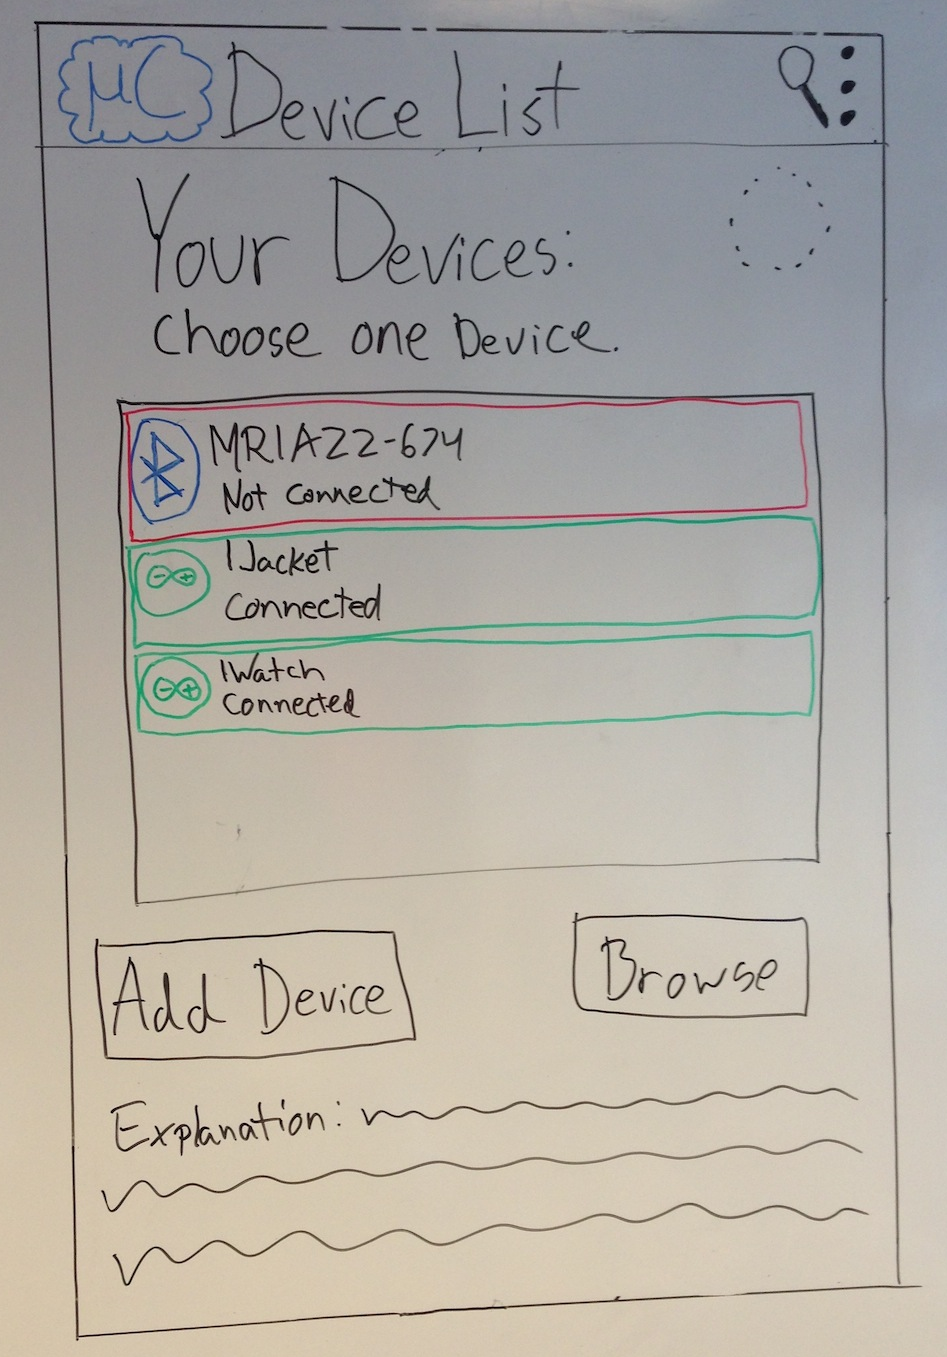
\includegraphics[scale=0.2]{images/Design_guide/Screen1a.png}
\caption{Screen 1a - Device list}
\end{figure}


\paragraph{Screen 1b - Add device manually}
Screen that appears after pressing the ''Add device'' button in Screen 1a. It was chosen to remove the ''Bluetooth settings'' button, as it unnecessary. In the final design, this screen contains only the ''QR code'' button and ''Input serial'' button, with a short description of the functionality of the button between them.

\begin{figure}[H]
\centering
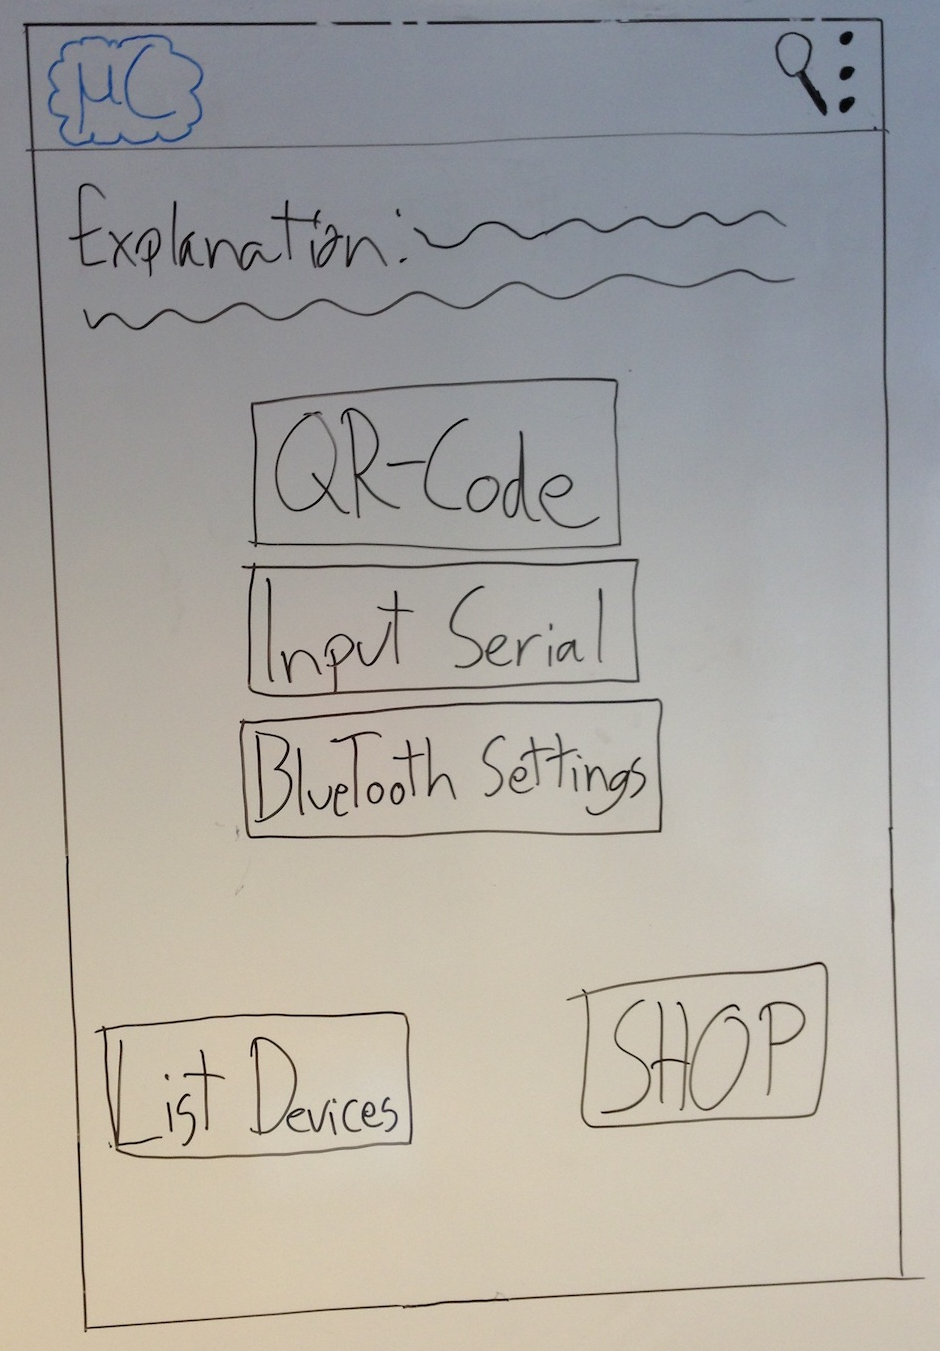
\includegraphics[scale=0.2]{images/Design_guide/Screen1b.png}
\caption{Screen 1b - Add device manually}
\end{figure}


\paragraph{Screen 1b-i - Input serial}
%Link to Screen 1b-i
Screen that appears when the ''Input serial'' button is clicked.

\begin{figure}[H]
\centering
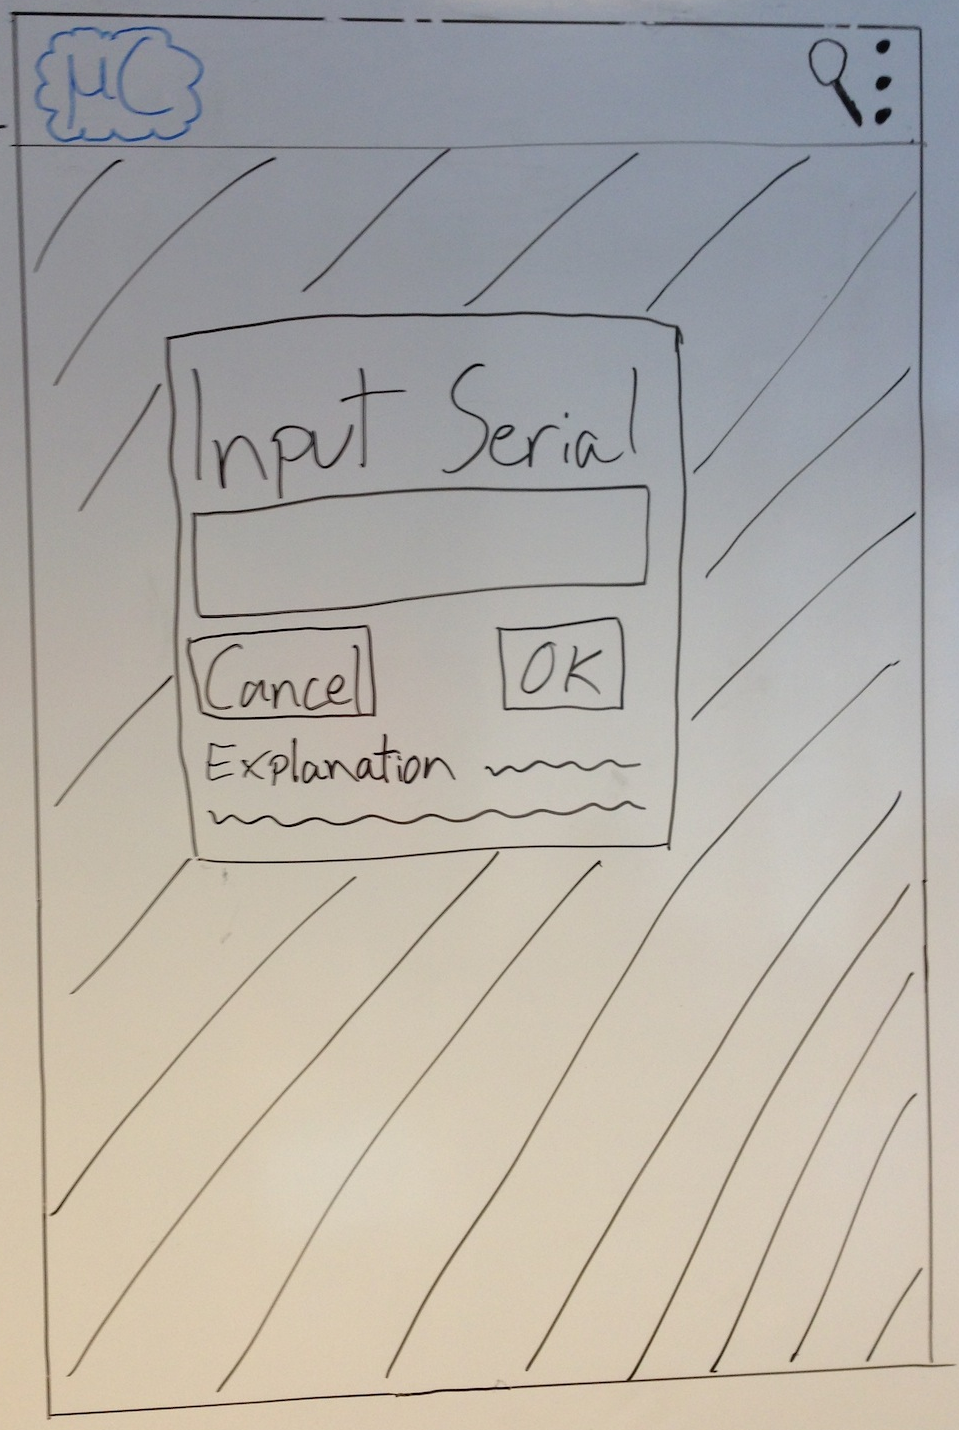
\includegraphics[scale=0.2]{images/Design_guide/Screen1b-i.png}
\caption{Screen 1b-i - Input serial}
\end{figure}


\paragraph{Screen 2a - Browse shop}
%Link to Screen 2a
Screen for browsing all the applications for Arduino in the shop. More categories have been added. The user can here swipe left/right to sort the available applications in different ways. See next paragraph.

\begin{figure}[H]
\centering
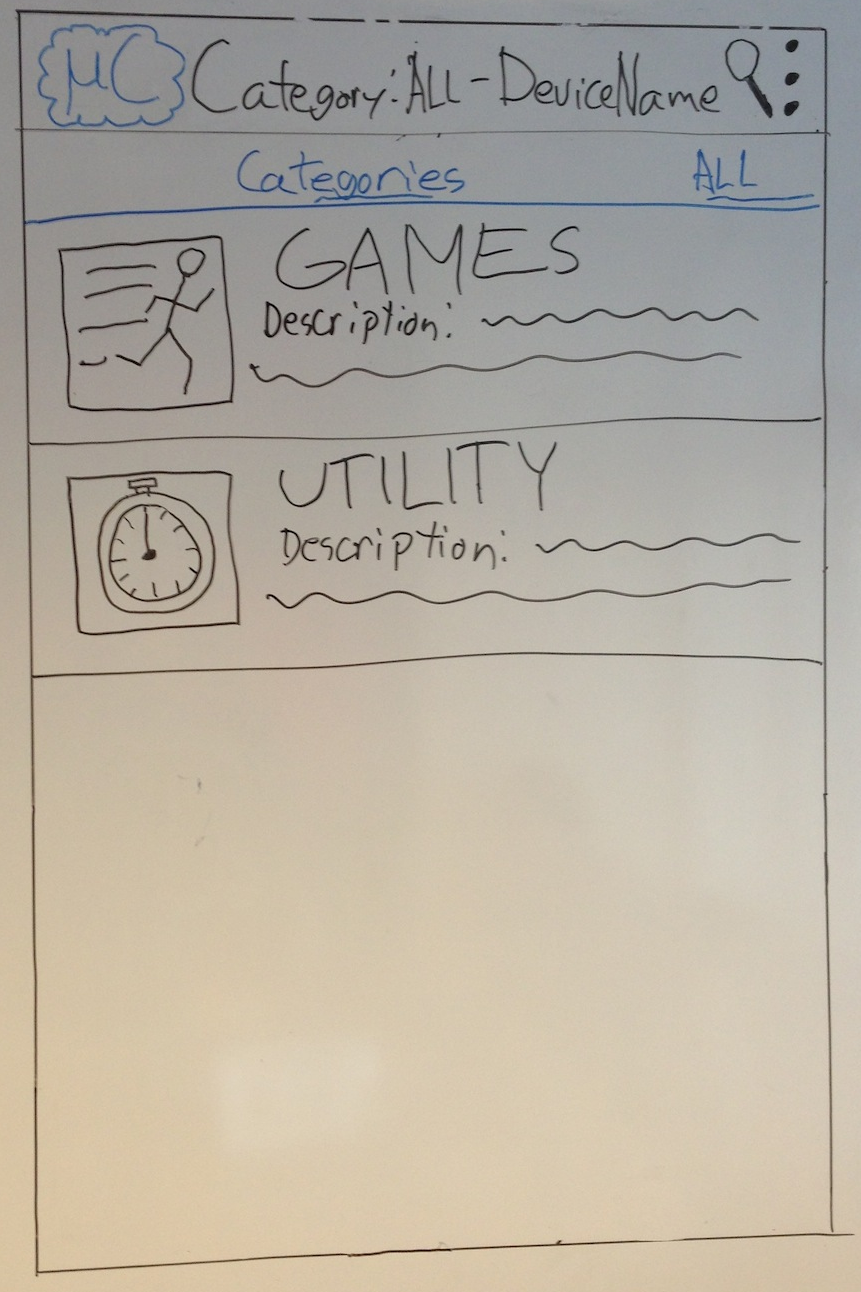
\includegraphics[scale=0.2]{images/Design_guide/Screen2a.png}
\caption{Screen 2a - Browse shop}
\end{figure}


\paragraph{Screen 2b - Browse shop by category}
%Link to Screen 2b
Screen that shows a list of all applications in chosen category. Category ''All'' is chosen.

\begin{figure}[H]
\centering
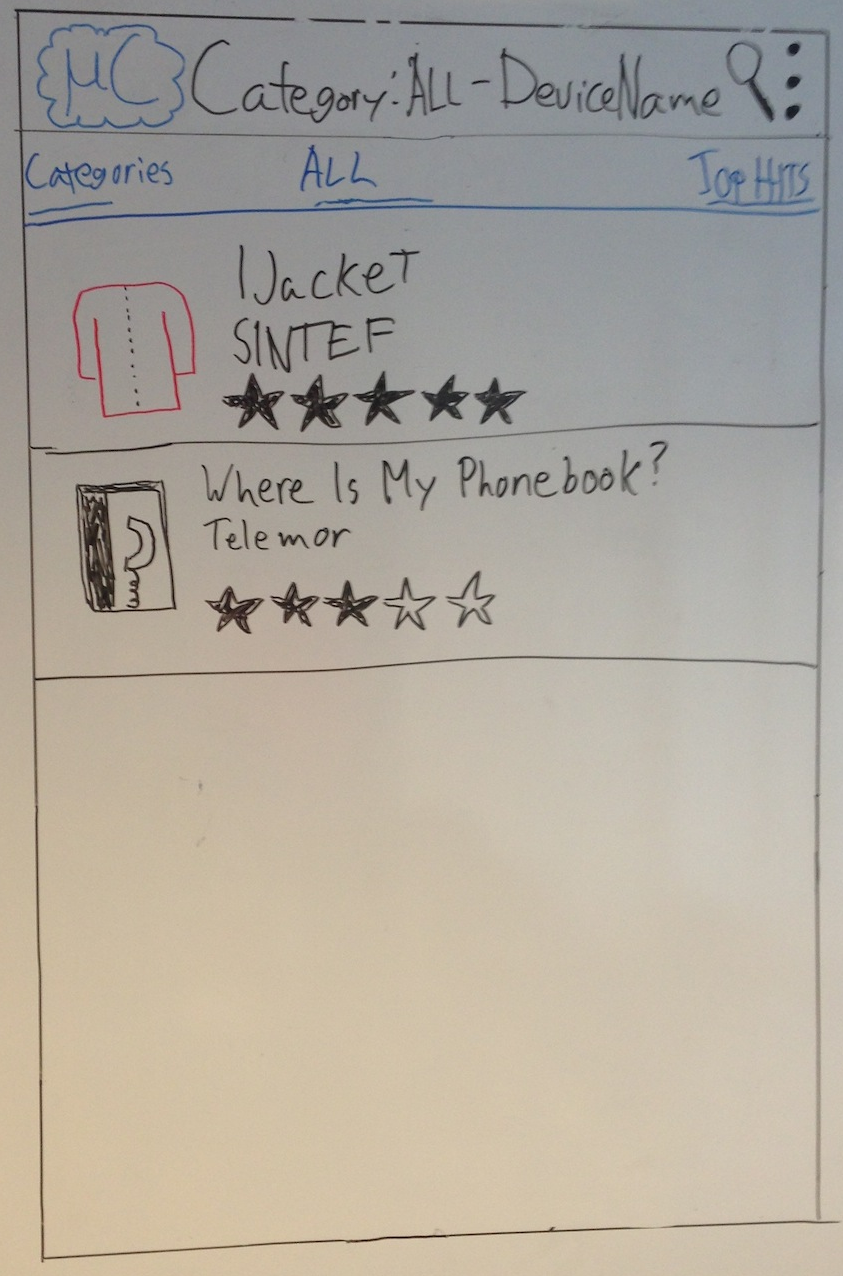
\includegraphics[scale=0.2]{images/Design_guide/Screen2b.png}
\caption{Screen 2b - Browse shop by category}
\end{figure}


\paragraph{Screen 3a - Application view}
%Link to Screen 3a
Screen with overview of an chosen application. Small changes were as comments field and reviews were given a lower priority at mid-term. 

\begin{figure}[H]
\centering
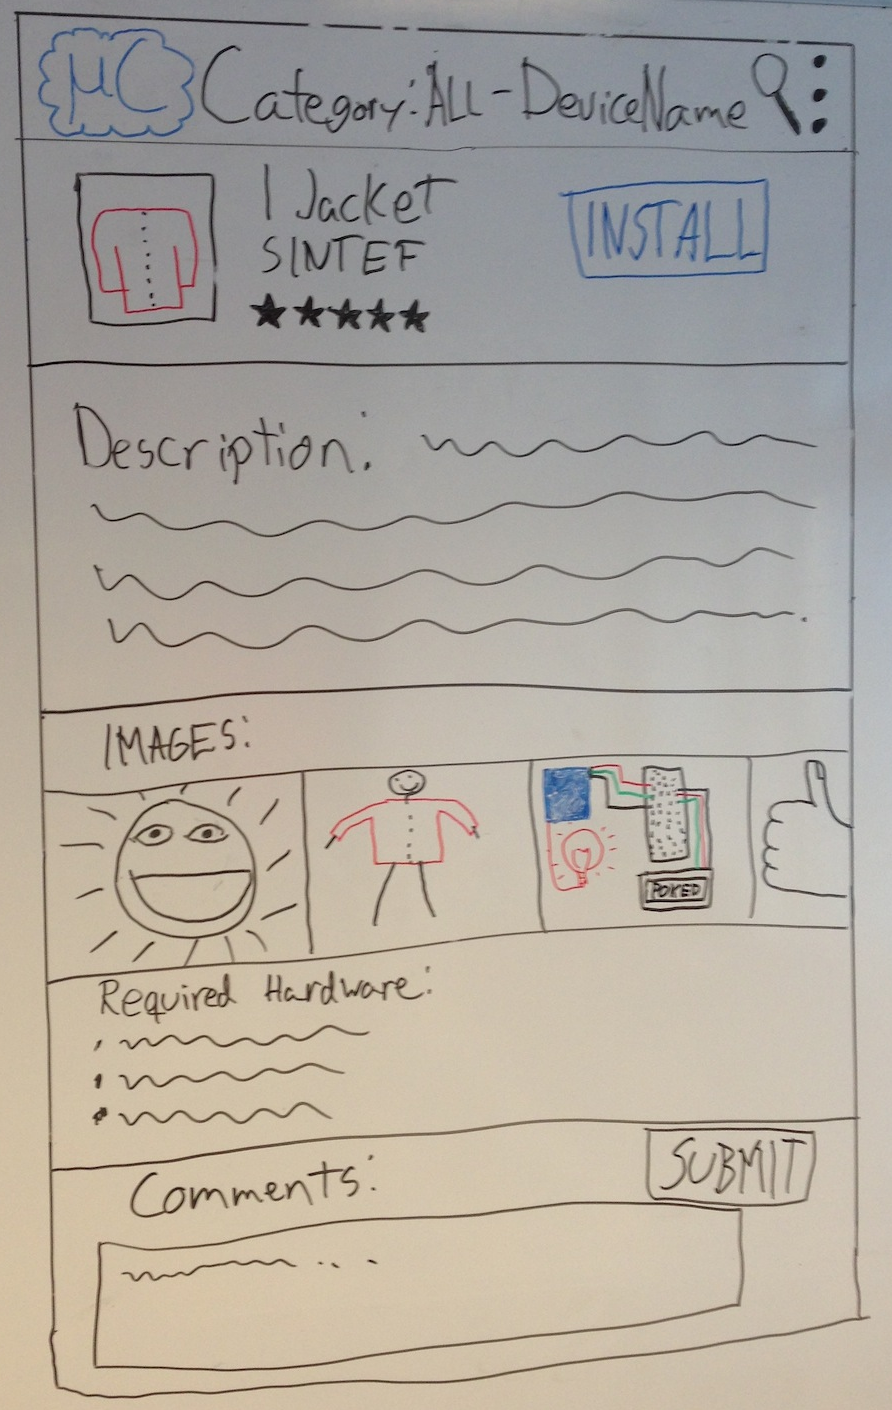
\includegraphics[scale=0.2]{images/Design_guide/Screen3a.png}
\caption{Screen 3a - Application view}
\end{figure}


\paragraph{Screen 3a-i - Installation confirmation}
%Link to Screen 3a-i
Screen that appears when the ''Install'' button in Screen 3a is pressed. Shows the name of the chosen device.

\begin{figure}[H]
\centering
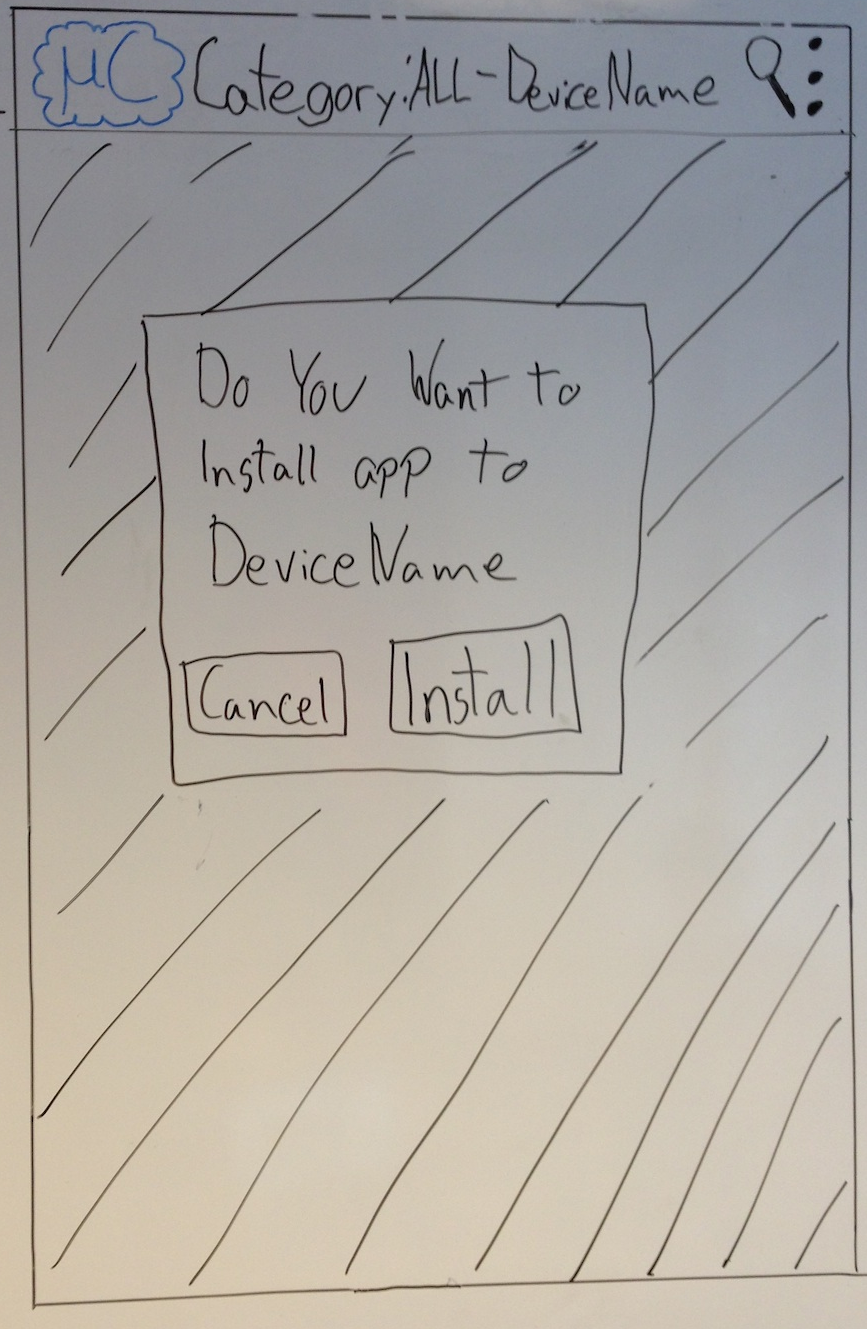
\includegraphics[scale=0.2]{images/Design_guide/Screen3a-i.png}
\caption{Screen 3a-i - Installation confirmation}
\end{figure}


\paragraph{Screen 3a-ii - Progress of installation}
%Link to Screen 3a-ii
Screen that shows the progress of the installation. The progress bar cannot be dismissed, so the Android application is locked until the installation is complete or has failed. 

\begin{figure}[H]
\centering
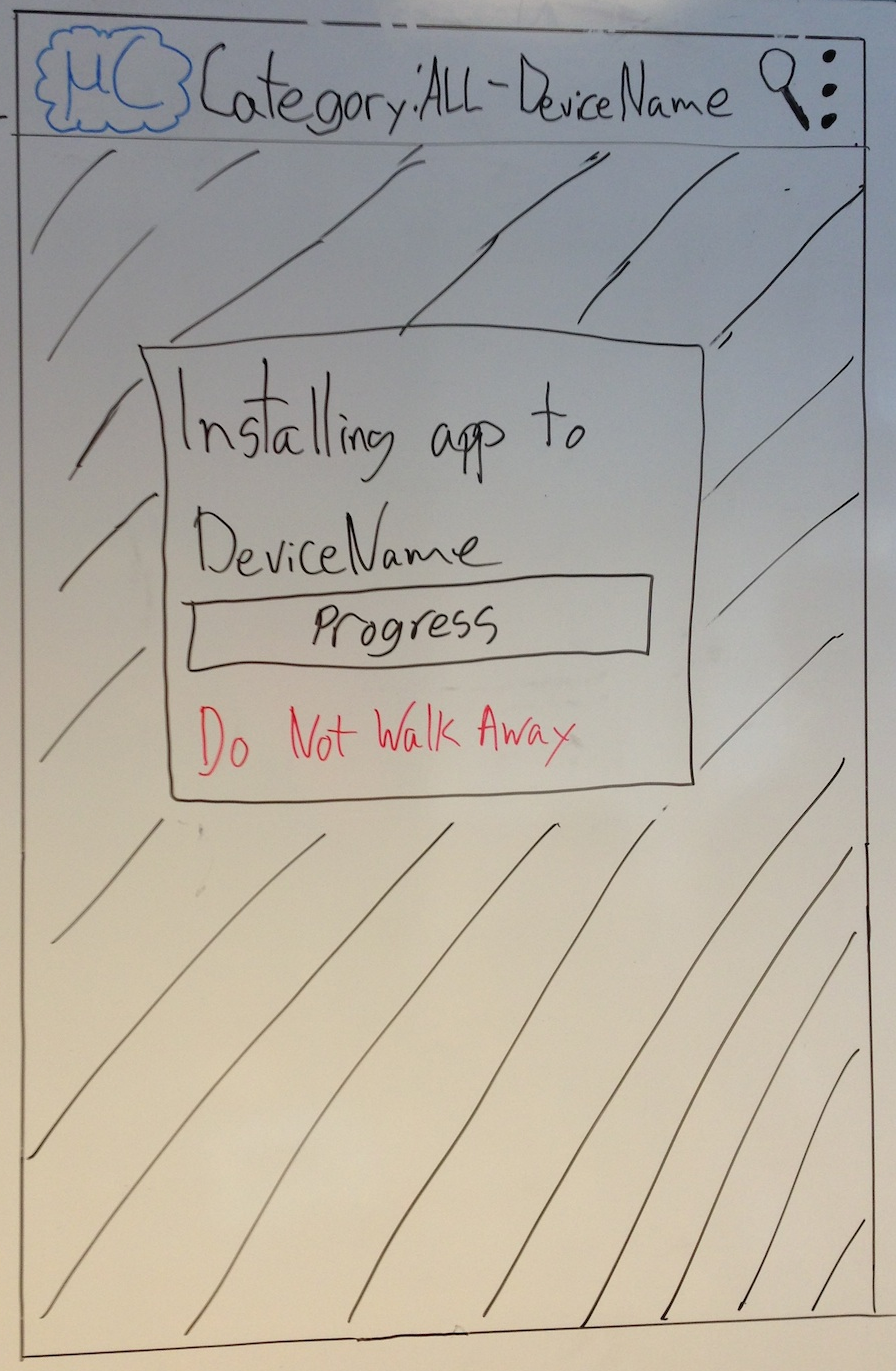
\includegraphics[scale=0.2]{images/Design_guide/Screen3a-ii.png}
\caption{Screen 3a-ii - Progress of installation}
\end{figure}


\paragraph{Screen Xa - Action overflow}
%Link to Screen Xa
Screen that appears when the ''Action overflow'' button is clicked. This menu is available from all the screen in the application with the exception of the preferences screen.

\begin{figure}[H]
\centering
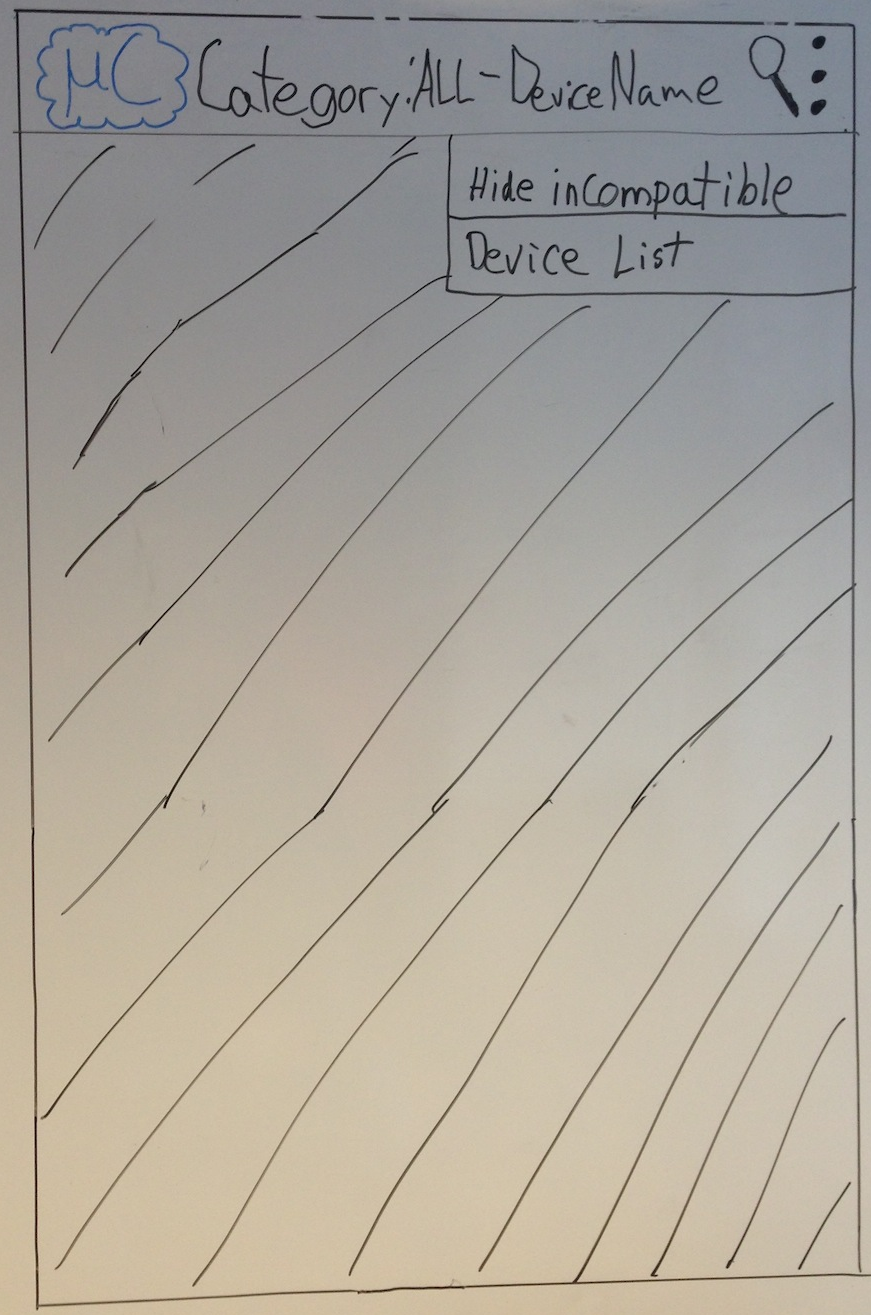
\includegraphics[scale=0.2]{images/Design_guide/ScreenXa.png}
\caption{Screen Xa - Action overflow}
\end{figure}
